\documentclass[a4paper,10pt]{article}

\usepackage[utf8]{inputenc}
\usepackage[french]{babel}
\usepackage{array,multirow,makecell}
\usepackage{color}
\usepackage{graphicx}
\usepackage{wrapfig}
\usepackage{hyperref}
\usepackage{fancyhdr}
\usepackage{fancybox}
\usepackage[squaren,Gray,cdot]{SIunits}
\usepackage{amsmath}
\usepackage{amssymb}
\usepackage{wasysym}
\usepackage{tikz}
\usepackage[tikz]{bclogo}
\usepackage{xkeyval}
\usepackage{ifthen}
\usepackage{ifpdf}
\usepackage{etoolbox}
\usepackage{mdframed}
\usepackage{xcolor}
\usepackage{tcolorbox}
\usepackage[a4paper,landscape,left=1.1cm,right=1.1cm,top=1.8cm,bottom=1.5cm]{geometry}\twocolumn
\usepackage{multicol}
\setlength{\columnseprule}{0.5pt}
\setlength{\columnsep}{25pt}

\def\d{\displaystyle}
\def\o{\overrightarrow}
\def\tr{\textcolor{red}}
\def\tb{\textcolor{blue}}
\def\tv{\textcolor{green}}
\def\tm{\textcolor{magenta}}
\definecolor{orange}{rgb}{0.99,0.69,0.07}
\definecolor{forestgreen}{rgb}{0.13,0.54,0.13}
\def\to{\textcolor{orange}}
\def\r{$\rightarrow\ $}
\def\tw{\textcolor{white}}
\def\so{\underline}
\def\su{\overline}
\def\esp{\vspace{0.2cm}}
\def\manip{\bcpanchant\ }


\newcounter{testcount} 
\newcommand{\test}{\stepcounter{testcount}
\noindent\bccrayon \textbf{\,Test \arabic{testcount}.} }

\newcounter{definitioncount} 
\newcommand{\defi}{\stepcounter{definitioncount}
\noindent\bccoeur \textbf{\,Definition \arabic{definitioncount}.} }

\newcounter{methodecount} 
\newcommand{\meth}{\stepcounter{methodecount}
\noindent\bcoutil \textbf{\,Méthode \arabic{methodecount}.} }

\setlength{\logowidth}{10pt}

\renewcommand{\theenumi}{\alph{enumi}.}
\renewcommand{\labelenumi}{\theenumi}
\renewcommand\thesection {\Roman{section} -}
\renewcommand{\thesubsection}{\hspace{0.5cm}\arabic{subsection})}
\renewcommand{\thesubsubsection}{\hspace{1cm}\alph{subsubsection})}

\renewcommand\bcStyleTitre[1]{\textbf{#1}}


\lhead{PCSI 2024 - 2025}
\rhead{TP physique - documents}
\chead{instruments en électricité - oscilloscope}
\cfoot{\thepage}

\pagestyle{fancy}

\date{}

\begin{document}


\thispagestyle{fancy}


\begin{center}
\begin{tcolorbox}[arc=1ex, colback=lightgray, colframe=black, left=3pt, right=3pt, top=3pt, bottom=2pt]
\begin{LARGE}
\begin{center}
\textbf{Oscilloscope  : METRIX DOX 2040}
\end{center}
\end{LARGE}
\end{tcolorbox}
\end{center}




\begin{center}
 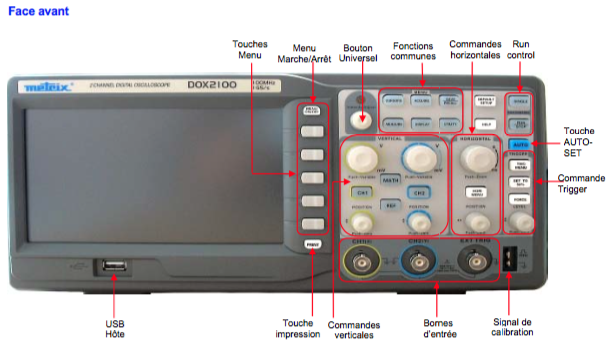
\includegraphics[scale=0.6]{oscillo-1.png}
 \end{center} 

\begin{center}
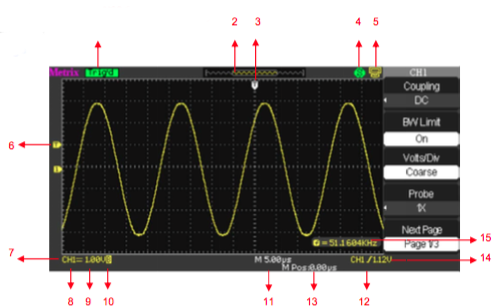
\includegraphics[scale=0.75]{oscillo-2.png}
\end{center}
 
\begin{center}
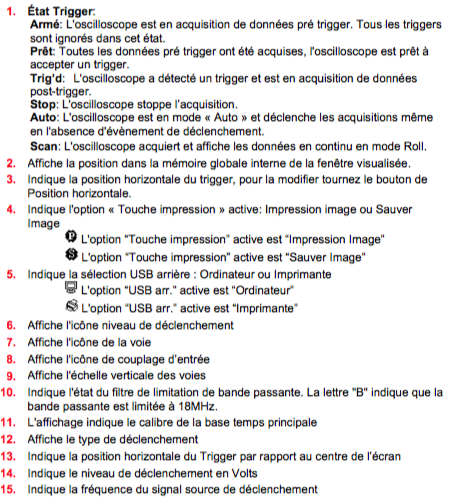
\includegraphics[scale=0.85]{oscillo-3.png}
\end{center}
 
\begin{center}
 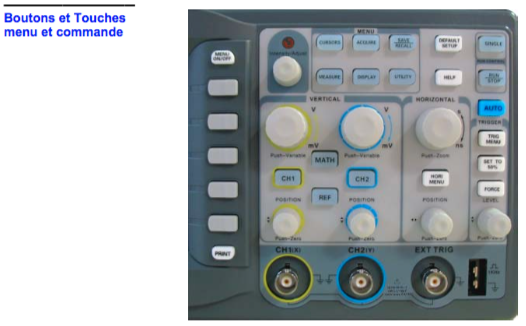
\includegraphics[scale=0.6]{oscillo-4.png}
 \end{center} 

\begin{center}
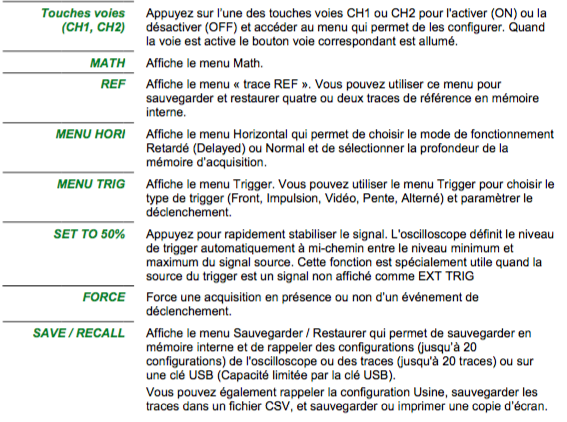
\includegraphics[scale=0.65]{oscillo-5.png}
\end{center}
 
\begin{center}
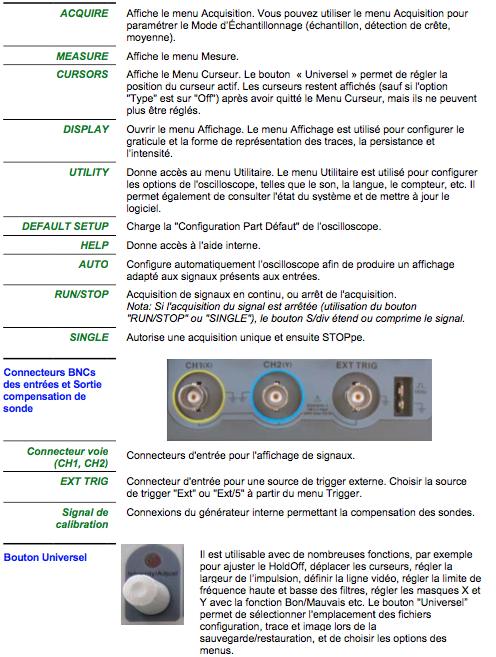
\includegraphics[scale=0.75]{oscillo-6.png} 
\end{center}



\end{document}